\documentclass{article}
\usepackage[utf8]{inputenc}
\usepackage{graphicx,caption}
\graphicspath{ {./images/} }
\usepackage{amssymb}
\usepackage{float}
\usepackage{breqn}
\usepackage{seqsplit}
\usepackage{titling}
\usepackage{changepage}
\usepackage{csquotes}
\usepackage{seqsplit}
\usepackage{hyperref}
\setlength{\parskip}{1em}
\addtolength{\skip\footins}{2pc plus 5pt}

\newcommand{\eq}[1]{{\ttfamily\seqsplit{#1}}}

\begin{document}

\begin{titlepage}
    \begin{center}
      \vspace{1.5cm}\Huge\textbf{Bitcoin and Elliptic Curves}\\
      \LARGE\textit{Understanding how cryptocurrencies work}\\
      \vspace{2cm}\Large\textbf{Fabio Dainese \hfill Nikita Baldan \hfill Marco Busato}\\
      \vspace{0.75cm}\Large\textit{Ca’ Foscari, University of Venice}\\
      \vspace{0.75cm}\Large March 13, 2019\\
      \vspace{2cm}\large\textit{\textbf{Keywords}: Bitcoin, Elliptic Curves, Cryptocurrencies, Security, Economy}
   \end{center}
   \let\thefootnote\relax\footnote{\textbf{Fabio Dainese} (email: \href{mailto:857661@stud.unive.it}{857661@stud.unive.it} or \href{mailto:dainese96@hotmail.it}{dainese96@hotmail.it}), \textbf{Nikita Baldan} (email: \href{mailto:857172@stud.unive.it}{857172@stud.unive.it}), \textbf{Marco Busato} (email: \href{mailto:852074@stud.unive.it}{852074@stud.unive.it}) - Master degree in 'Software Dependability and Cyber Security' (\href{www.unive.it}{www.unive.it}).}
\end{titlepage}

\section*{Preview}
\subsection*{Bitcoin}
A Bitcoin is a set of concept and technologies that form the basis of a digital money ecosystem. The Bitcoin are units of currency and they are used to store and transmit value among participants in the Bitcoin network. Users communicate using Bitcoin protocol, principally, via the internet. The Bitcoin protocol stack, that is available as open source software, can be run on a widely range of devices, including smartphones, that makes this technology vary accessible and portable.\newline
User can use Bitcoin to do anything that can be done with conventional currencies, such as: sell and buy goods, sent money to another user, people or organization or extend credit. Bitcoin can be purchased, sold and exchanged. Bitcoin are entirely virtual, this means that there's no existing physical coins. Users of Bitcoin own keys, that are stored in a digital wallet often stored on each user’s pc, to prove the ownership of Bitcoin in a Bitcoin network. With these keys they can sign transactions to unlock the value (BTC) and spend it by transferring it to a new owner.\newline
Bitcoin is a distributed, peer-to-peer system, so there isn’t a central server or point of control. They are created through a process called “mining”. Any user in a Bitcoin network can be a miner, only by using their computer’s processing power to verify and record transactions.\newline
The Bitcoin protocol includes built-in algorithm that regulate the mining function across the network. It also halves the rate at which new Bitcoin are created every 4 years, and limit the total number of Bitcoin that will be created to a fixed total (below 21 million coins).\newline
Due to Bitcoin’s diminishing rate of issuance, this currency is deflationary (which means that the value of Bitcoin increase). Furthermore, Bitcoin cannot be inflated by “printing” new money above and beyond the expected issuance rate.\newline
In other words: less is the number of Bitcoin in the network, much more is the user’s purchasing power and the value of currency increase. Bitcoin consists of:
\begin{itemize}
    \item Bitcoin protocol, a decentralized P2P network;
    \item Blockchain, which is a public chain that records the Bitcoin’s transaction;
    \item Consensus rule, rules for independent transaction validation and currency issuance;
    \item Proof-of-Work, which is a mechanism for reaching global decentralized
consensus on the valid Blockchain.
\end{itemize}
\begin{figure}[H]
    \centering
    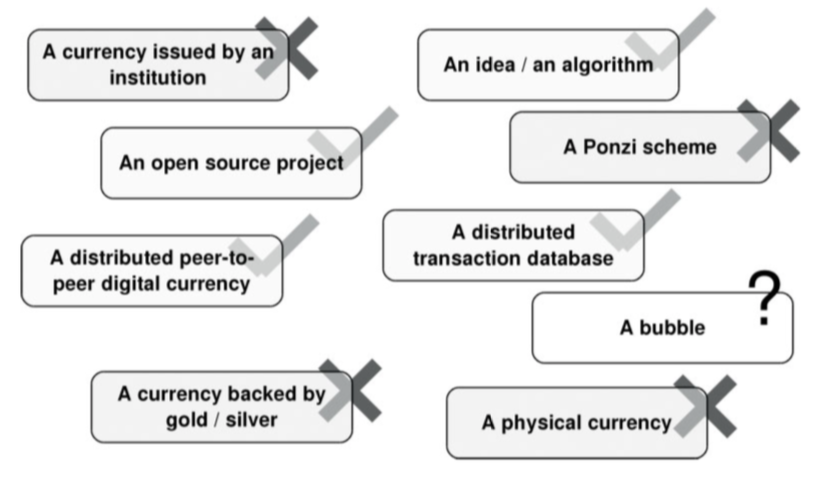
\includegraphics[width=8cm]{images/1.png}
    \caption{What Bitcoin is (and isn’t)}
\end{figure}

\subsection*{Elliptic Curves}
Let \(p\) be a prime number, and let \(\mathbb{F}_{p}\) denote the field of integers modulo \(p\). An elliptic curve \(E\) over \(\mathbb{F}_{p}\) is defined by an equation of the form:
\[ y^2 = x^3 + ax + b \]
where \(a, b \in \mathbb{F}_{p}\).\newline
The polynomial that we are taking into consideration is that one of the Weierstrass normal form of cubic curves. This rule says that, any cubic with a rational point can be transformed into the Weierstrass Normal Form (\( y^2 = x^3 + ax + b \)). The polynomial of degree 3, \( p(x) = x^3 + ax + b \) has at least a real root \(\alpha\) and two complex roots \(\beta, \gamma\). So we can rewrite the polynomial in the following way: \[p(x) = (x - \alpha)(x - \beta)(x - \gamma)\]\newline 
where \(\beta=-\alpha\beta\gamma;\hspace{1cm} \alpha=\alpha\beta+\alpha\gamma+\beta\gamma;\hspace{1cm} 0=\alpha+\beta+\gamma\).\vspace{5mm}\newline
The discriminant of \(p(x)\) is defined as follows:\newline
\[\Delta(p) = (\alpha - \beta)^2(\beta - \gamma)^2(\gamma - \alpha)^2\]\newline
An elliptic curve \(E\) is a non-singular cubic \(\{(x, y) : y^2 = x^3 + ax + b\} \cup \{\mathcal{O}\}\) where \(\mathcal{O}\) is a point at infinity and \(p(x)\) has three distinct roots iff the discriminant of the polinomyal \(\Delta(p) \neq 0\).
\paragraph{Examples:} Taking in consideration an elliptic curve of the form:
\[y^2 = x^3 + ax + b\]
with \(a = 0\) and \(b = 7\), which is actually the curve used by Bitcoins:

\begin{figure}[H]
    \centering
    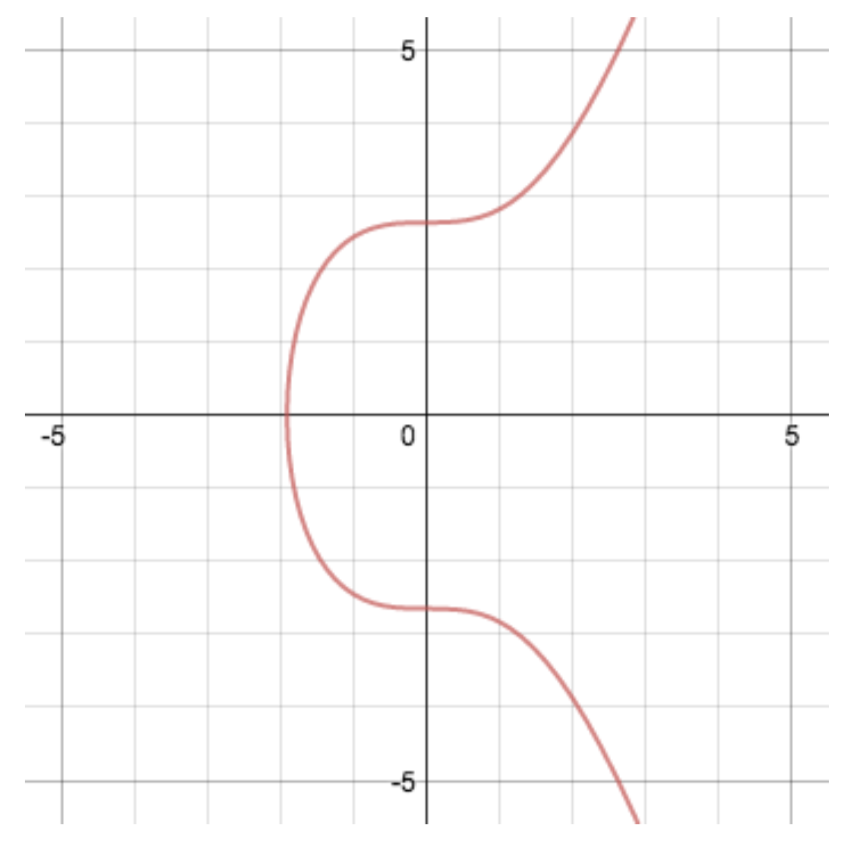
\includegraphics[width=8cm]{images/2.png}
    \caption{Elliptic curve used by Bitcoin}
\end{figure}

\noindent Elliptic curves have useful proprieties. For example, a non-vertical line intersecting two non-tangent points on the curve, will always intersect a third point on the curve. A further property is that a non-vertical line tangent to the curve at one point will intersect precisely one other point on the curve.\newline
We can use these proprieties to define two operations.\newline
\paragraph{Point addition:} Given the elliptic curve \(E\) and two points \(P\) and \(Q\) we can say that \(P + Q = R\) is defined as the reflection through the x-axis of the third intersecting point \(R\) on a line that includes \(P\) and \(Q\).

\begin{figure}[H]
    \centering
    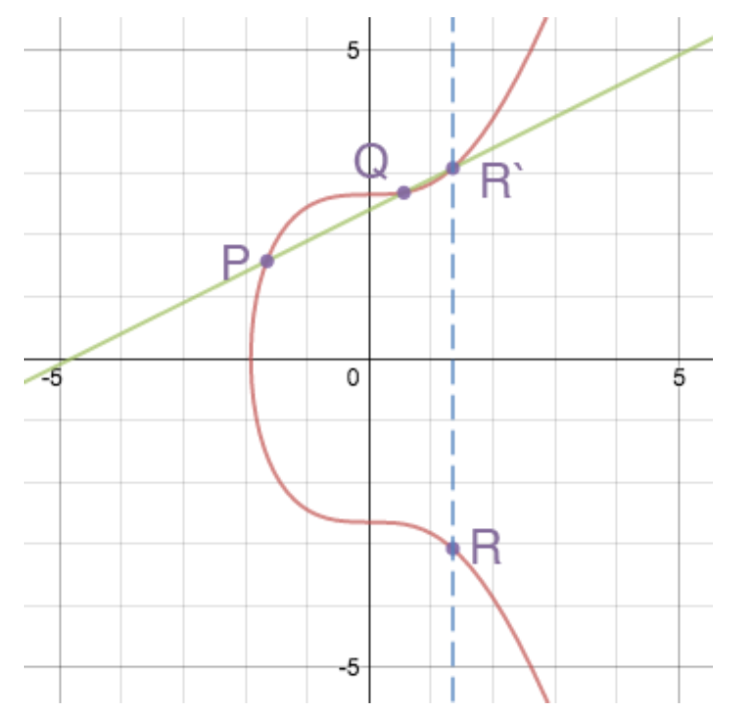
\includegraphics[width=7cm]{images/3.png}
    \caption{Elliptic curve point addition}
\end{figure}

\paragraph{Point doubling:} Given the elliptic curve \(E\) and a point \(P\), we can say that \(P + P = R\) is defined by finding the tangent line to the point \(P\), and taking the reflection through the x-axis of the intersecting point \(R\) on the curve to get \(R\).

\begin{figure}[H]
    \centering
    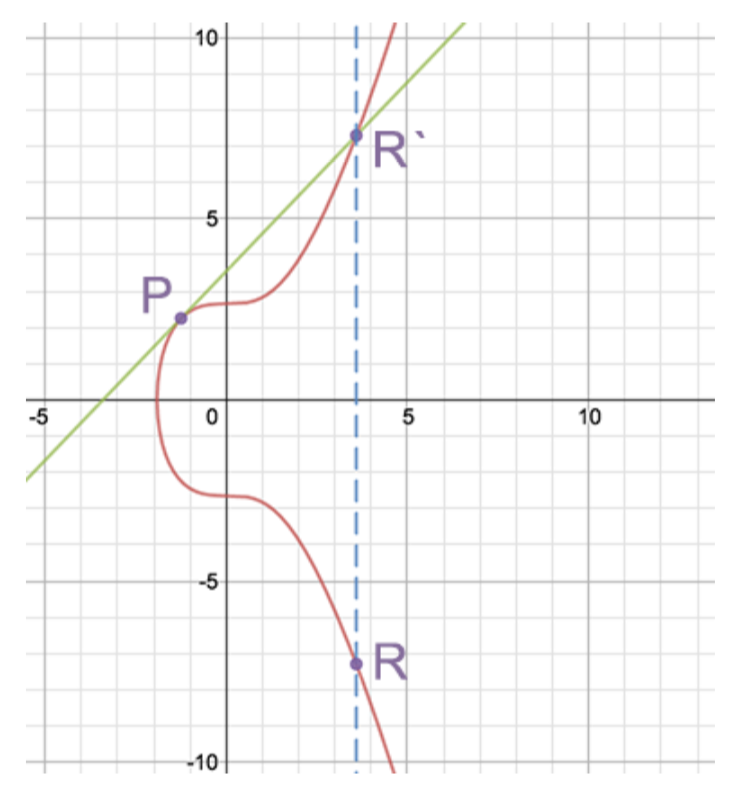
\includegraphics[width=7cm]{images/4.png}
    \caption{Elliptic curve point doubling}
\end{figure}

\noindent These two operations are used for scalar multiplication, \(R = aP\). For example:
\begin{adjustwidth}{2.5em}{0pt}
    \(R = 7P\)\newline
    \(R = P + 6P\)\newline
    \(R = P + 2 (3P)\)\newline
    \(R = P + 2 (P + 2P)\)
\end{adjustwidth}
Here, \(7P\) has been broken down into two point doubling steps and two point addition steps.

\subsection*{Finite Field}
A finite field, in the context of ECDSA (Elliptic Curve Digital Signature Algorithm), can be thought of as a predefined range of positive numbers within which every calculation must fall. Any number outside this range “wraps around” so as to fall within the range.\newline
Combining the usage of elliptic curves and finite fields, maintains the proprieties of the elliptic curves, but having a finite number of points.\par 
\noindent The curve taken in consideration before \((y^2 = x^3 + 7) \bmod 67\) will look like the following picture:

\begin{figure}[H]
    \centering
    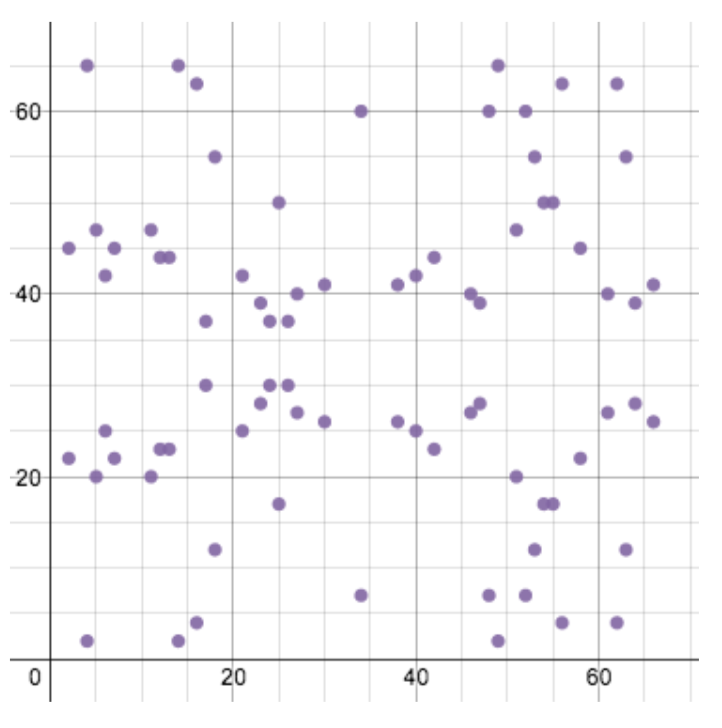
\includegraphics[width=7cm]{images/5.png}
    \caption{Representation of \((y^2 = x^3 + 7) \bmod 67\)}
\end{figure}

\noindent We can see that the previous curve is now a set of points, in which \(x\) and \(y\) varies from \(0\) to \(66\).
\clearpage

\section*{Introduction}
Bitcoin is a decentralized digital currency, it is based on a peer-to-peer network of computers running the software. These computers are called nodes. Partecipants in the network might be running nodes for different reasons: for profit as the case of miners, to manage full-node wallets, to collect and study informations about the network or simply as a social good.\newline
Bitcoin’s decentralized nature contrasts to the structure of fiat currencies.\newline
Fiat money is a currency without intrinsic value that has been established as money, often by government regulation.\newline
Central banks make monetary decisions after evaluating evidence gathered from the evolution of the economy. In a decentralized system such as Bitcoin, discretionary decisions are not possible. The original creators of the system have to take most of the decisions upfront at the design phase. These decisions have to be carefully balanced, and take into account the incentives of the different users, otherwise the decentralized system is doomed to fail. In Bitcoin, the monetary policy follows a simple rule: the final monetary base is fixed at around 21 million Bitcoins and new BTC are minted at a planned schedule and paid to users who help secure the network. This serves the double purpose of providing the Bitcoins with value due to their scarcity and creating incentives for users to connect to the network and help secure it by providing their computational power.\newline
Another feature of decentralized systems is their resilience. Decentralized systems are robust against attacks either by insiders or by external forces. This feature might have been critical for the existence of Bitcoin. Earlier centralized attempts to create digital currencies were forced down by governments. However, to force down a decentralized system, all individual users must be forced down, which is a much harder task. Bitcoin’s peer-to-peer nature makes it also censorship-resistant.\newline
The main technological breakthrough accomplished by Bitcoin is solving the double-spending problem in a distributed financial database. A double-spend attempt occurs when a user tries to spend some funds twice. All financial systems must reject these attempts. This is relatively straightforward in a centralized system, as transactions are recorded in a central database and future spending attempts are checked against this database first. In a decentralized system, many copies of the database are shared among the peers, and keeping a consistent state of the database is a difficult computational problem (Byzantine Generals’ problem). In the context of Bitcoin the problem is how the network can agree on the state of the distributed database when messages between the nodes can be corrupted and there might be attackers trying to subvert the distributed database. Bitcoin gracefully solves this problem that will be analyzed in detail in the next sections.
\subsection*{Open Source}
Bitcoin is open source software, which means that the source code is available for anyone to use, modify, and redistribute free of charge. The difference between open source software and proprietary software lies in their licenses. A proprietary software license grants the right to use a copy of the program to the end user. However, ownership of the software remains with the software publisher. In contrast, an open source license, as we said earlier,  grants the user the right to use, copy, modify, and redistribute the software. The copyright of the software remains with the creator, but the creator of an open source software transfers the rights to the user as long as the obligations of the license are met. Another difference between proprietary and open source programs is that proprietary programs are usually distributed as compiled binaries. This means that the software is usually distributed in machine language. Users willing to gain knowledge on what the software is doing must interpret the machine code in a time-consuming process called reverse engineering while in a open source software the user can directly have access to the source code.\newline
Proprietary software requires that the company issuing the software maintains and updates it; under an open source license it is legitimate to start a new independent software project from a copy of an original one. This process is called forking. The threat of a fork can often keep the developers of an open source project honest. If the developers of a project introduce changes that are detrimental to the users of the software, anybody can create a fork, undo those changes and continue the development.
\subsection*{Peer-to-peer (P2P)}
In a P2P network, the "peers" are computer systems which are connected to each other via the Internet. Files can be shared directly between systems on the network without the need of a central server. In other words, each computer on a P2P network becomes a file server as well as a client.\par
\noindent The only requirements for a computer to join a peer-to-peer network are an Internet connection and P2P software. Common P2P software programs include Kazaa, Limewire, BearShare, Morpheus, and Acquisition. These programs connect to a P2P network, such as "Gnutella," which allows the computer to access thousands of other systems on the network.\par
\noindent Once connected to the network, P2P software allows you to search for files on other people’s computers. Meanwhile, other users on the network can search for files on your computer, but typically only within a single folder that you have designated to share. While P2P networking makes file sharing easy and convenient, is also has led to a lot of software piracy and illegal music/video downloads.

\subsection*{Centralized Database}
The main problem in transfer money with a system such as Bitcoin, it is to avoid double spending.\newline
An example of double spending is the following: Say Alice has a digital coin, represented by the binary number 01000101. She could transfer this value to Bob, by sending him a message with this number, so that Bob had a copy of the number and thus the value. The problem is obviously that nothing prevents Alice from sending this same number to another user or indeed to many other users. As we can see from this example, digital value cannot be represented as a number because digital data is very easy to replicate many times.
\begin{figure}[H]
    \centering
    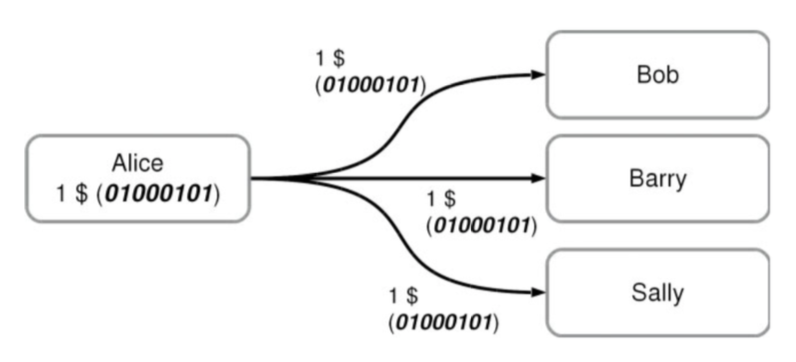
\includegraphics[width=8cm]{images/6.png}
    \caption{Double spending problem}
\end{figure}

\par\noindent The next step towards building a digital payment system is to create a central database, holding a list of the users and the funds held by any of them. Now if Alice wants to transfer 1 unit of the currency, say a token, represented by the number 01000101 to Bob, she contacts the server running the central database and directs it to transfer this token to Bob. The server updates the database, and the token now belongs to Bob. If Alice tries to double-spend the token 01000101, sending it to Barry this time, she would have to again connect to the central server and direct it to send the token to Barry. However, upon checking the database, the server sees that the token 01000101 does not belong to Alice anymore, and thus she is not authorized to spend it. So, as you have seen having a central database solves the double-spend problem easily.

\begin{figure}[H]
    \centering
    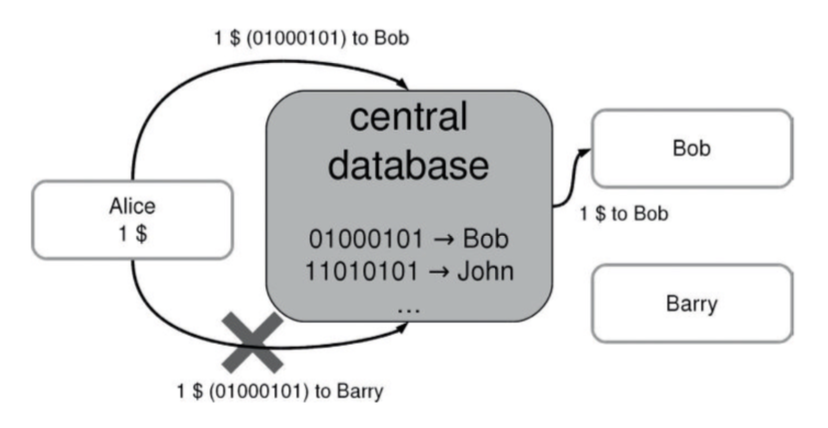
\includegraphics[width=8cm]{images/7.png}
    \caption{Centralized database}
\end{figure}

\noindent However, there are issues associated with a central database. For a start, all users must have previously registered with the central server in order to operate. Thus the central database knows the identities of all the users and collects their financial history. A central database is also an easy target to attack, either by insiders or by outsiders. If an attacker gets control of the central database, it could change the ownership of any funds, thus stealing them from their legitimate owners or create new funds and assign them to himself. \par
\noindent As you already known Bitcoin’s ledger database is distributed and maintained by many computers called nodes. Bitcoin users can send new transactions to this distributed database, where they are recorded. Both systems are resilient, even in scenarios where a large portion of the network is forced down.

\subsection*{Addresses and Transactions}
Bitcoins do not reside in user’s computer, but instead they are entries into the Blockchain,
that does not store accounts and balances but only transactions. This decentralized ledger basically contains all the transactions that have been made by every user since the beginning and by
analyze they each user can retrieve its balance. A transaction is composed of a list of transaction inputs (TxIn) and transaction outputs (TxOut). Each transaction output stores two values:
\begin{itemize}
    \item Amount;
    \item Recipient address, that is derived from the public key.
\end{itemize}
Only the owner of the private key can unlock the funds stored in the TxOut, to do this, the owner of the private key must sign a transaction sending the funds to a new Bitcoin address. Transaction input holds a reference to a previous transaction output, and a signature that proves that the funds in the previous TxOut it references can be spent.\newline
This signature must be done with the private key associated with the public key in the Bitcoin address. If the signature does not match the transaction is considered invalid and dropped by the network.\newline
The purpose of a transaction is to distribute the funds from the input to the output. Input in a transaction reference outputs in previous transaction. The output must not have been spent, otherwise the transaction is invalid.\newline
A transaction is considered valid if the sum of the amounts of the input is greater or equal to the sum of the amounts of the output.\newline
There is a difference between input and output transaction, and it is the fee of the transaction.\newline
The transaction fee is collected by the miners that include the transaction in a block.\newline
Output in the blockchain can be spent only once, and they must fully expended.\newline
If the amount of the outputs is greater than the amount to be spent, the transaction generates change and can be collected by the sender by adding a change address as an additional output of the transaction.\newline
The first node in the network that receives the transaction verifies that it is a valid transaction. If the transaction is correct, the node relays it to other nodes in the network. To verify that a transaction is valid, a node follows these steps:
\begin{itemize}
    \item It checks that the signatures for each of the inputs are valid, i.e. that each of the inputs is signed with the private key corresponding to the public key associated with the address it references. If one of the signatures is not correct, the nodes reject the message;
    \item It checks that the previous outputs referenced by the transaction exist, and that they have not been spent. The node carries this check by consulting the Unspent transaction outputs cache (UTXO);
    \item It checks that the sum of the values of the inputs is greater than or equal to the sum of the outputs. That is, it checks that the transaction is not spending more than the available inputs. The difference between the sum of the value of the outputs and the sum of the value of the inputs is considered to be the fee left for the miner, and it is included in the coinbase transaction. If there are not enough funds the transaction is considered invalid;
\end{itemize}
Bitcoin’s software maintains an unspent transaction outputs cache (UTXO).\newline
The UTXO is a database containing only the unspent transaction outputs and is very useful as it can be used to quickly check if new transactions are valid. When a new transaction arrives, its inputs are looked up in the UTXO. If all the inputs are found there then the inputs correspond to valid previous outputs, and the transaction continues to be evaluated. If any of the inputs are not found in the UTXO, the transaction is not valid and can be discarded.\par

\noindent As anticipated, Bitcoin identifies users by large alphanumeric strings such as “\textit{13mckXcnnEd4SE\allowbreak kC27PnFH8dsY2gdGhRvM}”. The address is the public part of a public–private cryptographic key. The private part of the key is under the control of the user.\par
\noindent An example of utilization of this system is used when a user (Alice) wants to send some funds to another user (Bob): \begin{displayquote} Alice uses her private key to sign a message that says “I want to send 1 Bitcoin to 1gr6U6...” and after that she sends it to the network.\end{displayquote} Note that Alice does not identify the user she wants to send funds to, just the address to receive the funds. Thus Alice must find out Bob’s address through other means.\par

\noindent An important detail is that the nodes in the network do not know the identities of either Alice or Bob, as users are identified only by their addresses. Bitcoin users are identified by a pseudonym: Bitcoin provides pseudonymity. Another important detail is that addresses are not granted by the network. They are created inside the users’ devices when it runs the Bitcoin software that generates the cryptographic public and private keys. No prior registration is necessary to use Bitcoin. In fact, new users do not even have to communicate their addresses to the network to be able to receive funds. A user, say Bob, can generate an address and communicate this address to Alice through other means, such as an email or the pairing of two smartphones. Alice can now send funds to Bob’s address and the network would accept the transaction even though it has never encountered that address before.\newline
In a centralized system the funds are held by a central entity, which also holds the means to control those funds, say by changing the registries in the ledger. In contrast, in a decentralized system, the private keys that give access to the funds are solely in the hands of the end users.

\subsection*{The Blockchain}
A Blockchain is a open and distributed digital register that can record data, called transaction, in a safe, verifiable and permanent way.\par\noindent
The blockchain uses proof-of-work to secure the distributed database. This means that the blockchain is secured against tamper attempts by the computational power that has been applied to create it. An attacker wishing to change the blockchain would have to apply a computational power equivalent to all the computational power spent from that point in time to the present, this because every block must be changed.\newline
For each block it is possible to associate more transaction. Each block contains:
\begin{itemize}
    \item Version, depends on the version of the used software;
    \item Hash of the previous block, hash of 256 bit that is necessary to link the
last block;
    \item Merkle root, hash of each hash in a block;
    \item Timestamp, timestamp of the last transaction;
    \item Bits, current target value;
    \item Nonce, 8 byte value that it is added in the block and it must be lower of
target value. The value is recalculated if the block hash does not contain
the required number of zero;
    \item Transaction number.
\end{itemize}
Nowadays it contains about 250 GBs of data and it is getting bigger. A particular feature of the Blockchain is that it is decentralized, so everyone in the Bitcoin network can keep it up-to-date.\par

\noindent There are software that parse the blockchain, like mining nodes or wallets, in order to extract relevant information, such as whether a particular transaction output is spendable or which is the current balance of the account.

\subsection*{Mining}
Mining is the mechanism by which Bitcoin’s security is decentralized.\newline
Miners validate new transaction and record them in the Blockchain. On the average a new block is “mined” every 10 minutes. By doing this, transactions are added to the blockchain as part of the block added, and considered “confirmed”, which allows the new owner to spend those Bitcoin.\newline
Miners receive two types of rewards: new coin created with each block, and transaction fees from all the transactions included in the block. To earn this rewards miners have to solve the Proof-of-Work problem.\par
\noindent We will describe in more accurate details the mining process and the involved technologies in the next sections.

\subsection*{Adding a Block (Proof-of-Work)}
To add a new block you need to solve a math problem called Proof-of-Work. The first user that solves the problem get to add the next block.\newline
The Proof-of-Work involves scanning for a value that when hashed, using SHA256, together with the other block's information its gives a string that's begins with a certain number of zero bits. The average work is exponential in the number of zero bits that are required to satisfy the problem.\newline
In order to solve this problem we cannot modify the values of the block (transactions ID) and that's why we have the nonce field in the block.\newline
The proof of work difficulty is determined by a moving average targeting number of blocks per hour. Remember the fact that the Proof-of-Work must produce a hash that is less than the target. A higher target means that it is less difficult to find the nonce value. A lower target means it is more difficult to find the nonce value.

\subsection*{Validate a New Block}
As the newly solved block moves across the network, each nodes perform a series of test to validate it before propagating it to its peers. This ensure that only valid block are propagated on the network. When a node receive a new block it checks that:
\begin{itemize}
    \item The block data structure is syntactically correct;
    \item The block header hash is less than the target (enforces the Proof-of-Work)
    \item The block timestamp is less than two hours in the future (allowing for
time errors);
    \item The block size is within acceptable limits;
    \item The first transaction (and only the first) is a coinbase transaction;
    \item All transaction within the block are valid using the transaction checklist.
\end{itemize}
The independent validation ensures that the miners cannot cheat. An invalid coinbase transaction would make the entire block invalid. For this reason miners have to construct a perfect block, based on the shared rules that all nodes follow, and mine it with a correct solution of the Proof-of-Work.\newline
To do so, they spend a lot of electricity in mining, and if they cheat, all effort and electricity is wasted. This is why independent validation is a key component of decentralized consensus.
\clearpage

\section*{Bitcoin Technology}
When we talk about cryptocurrency, we have to highlight the importance of cryptography in the currency design.\newline
Bitcoin originally makes use of three types of cryptography systems:
\begin{itemize}
    \item Public key cryptography. Bitcoin uses public key cryptography to handle transactions;
    \item Hash functions. Bitcoin uses hash functions to secure the information in the blockchain;
    \item Symmetric key cryptography. Bitcoin uses symmetric encryption to protect the private keys in a user’s wallet. The use of symmetric encryption in the wallet software is not a requirement.
\end{itemize}

\subsection*{Public Key Cryptography}
Public key cryptography was developed as a response to an important weakness of symmetric encryption: key distribution.\newline
When two people use symmetric encryption, they must ensure beforehand that they both share the same symmetric key: they must interchange the keys through a secure channel before using the symmetric encryption system. However, there are many situations where it is not possible to interchange the symmetric key through a secure channel, such as e-commerce. The internet is an insecure channel: traffic can be eavesdropped and even modified in transit. Therefore it is impossible to establish a secure connection through the internet using only symmetric encryption. Public key encryption was developed to overcome this problem. The best way to represent this problem is with an example.\newline
In the following picture, it is represented the public key encryption in action. In this example public key cryptography is used to encrypt a message. First, the receiver of the encrypted message (Bob) generates a pair of public and private keys, running a key generation algorithm (1). The public and private keys are called a public–private keypair and are mathematically linked. Every public key protocol has its own key generation algorithm. The receiver (Bob) sends his public key to the sender (Alice) (2) but keeps his private key secured. After receiving Bob’s public key, Alice proceeds to encrypt the message using Bob’s public key (3). The result is the encrypted message (ciphertext). This encrypted message is sent over the insecure channel to Bob (4). An attacker eavesdropping the connection can get hold of the encrypted message, but she cannot decrypt it. Only Bob, who has the private key corresponding to the public key, is able to decrypt the encrypted message using the decryption algorithm (5), obtaining the original message (6).

\begin{figure}[H]
    \centering
    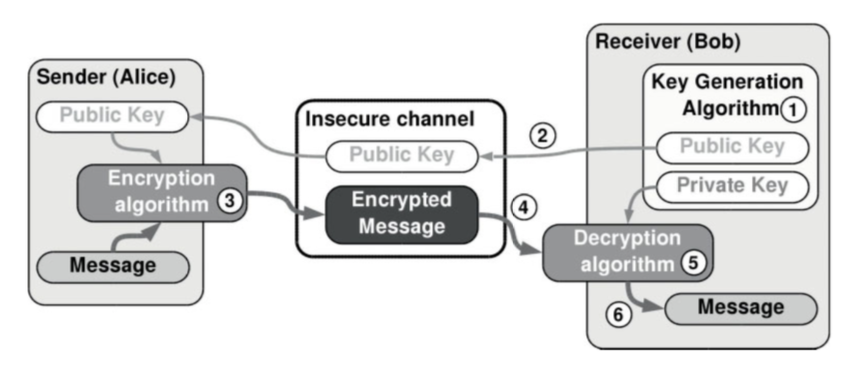
\includegraphics[width=8cm]{images/8.png}
    \caption{Public key encryption}
\end{figure}

\noindent There is a problem with the proposed encryption scheme: the public key is sent over the insecure channel. This opens the possibility of a Man-in- the-Middle attack (MitM). The attacker (Trudy) controls the communication channel. She can intercept a message flowing through the channel and change it before it is received. Trudy takes advantage of her position by intercepting the public key that Bob sends to Alice at the beginning of the communication (2). But she does not forward Bob’s public key to Alice, instead she keeps Bob’s public key to herself and generates a brand new public–private keypair (3). The keys controlled by Trudy show a dot next to them in Figure 9. Trudy then sends her own generated public key to Alice as if it were Bob’s public key (4). Later, when Alice wishes to send Bob an encrypted message, she encrypts the message with what she believes to be Bob’s public key (5). The encrypted message is intercepted by Trudy (6), and because it was encrypted with a public key of her own, she is able to decrypt the message (7). Trudy then proceeds to re-encrypt the message, this time using Bob’s public key (8). She then passes this second encrypted message to Bob (9). Bob is able to decrypt the message using his private key (10). Notice that during this attack neither Alice nor Bob have any indication that they are being attacked.

\begin{figure}[H]
    \centering
    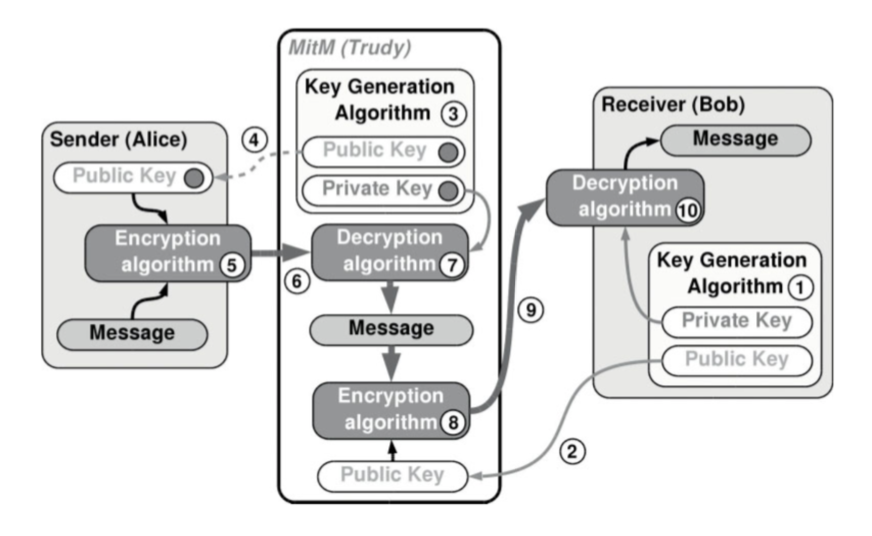
\includegraphics[width=8cm]{images/9.png}
    \caption{Man-in-the-Middle attack}
\end{figure}

\noindent To avoid this type of attacks there are several approaches:
\begin{itemize}
    \item Bob and Alice can interchange their public keys using a different, secure channel. The downside to this approach is that this is a similar problem (key distribution) to the problem that public key cryptography tries to solve;
    \item Web of trust. Users cryptographically sign the public keys of other users they know and trust, for instance because they have met face to face in a key-signing party. Every user keeps a keyring, a set of other users’ public keys. A user can cryptographically sign the public key of other users that she/he knows. If a user wishes to communicate with someone she does not know, she/he can ask any of her trusted friends;
    \item Public Key Infrastructure (PKI). PKI assumes there is a central authority, called the Certificate Authority (CA). Everybody has a copy of the CA public key, and trusts the CA. Every user generates a public–private key pair and presents at the CA its public key. The CA verifies the identity of the user and then signs its public key. When Alice wants to communicate with Bob, she sends her certificate to him, which comprises her public key and the CA signature for that public key. Bob then checks that Alice’s public key is properly signed by the CA, i.e. that the certificate is valid. This is the approach followed by SSL and TLS, the world’s largest cryptographic deployment.
\end{itemize}
TLS work in two steps. First, a symmetric key is randomly generated by one of the two ends, say Alice. Next this symmetric key is encrypted by Alice with the public key of the other end (Bob). The encrypted symmetric key is sent over the internet to Bob. Only Bob has the private key, so only he can decrypt the message and obtain the symmetric key generated by Alice. At this point both Alice and Bob have the same symmetric key. Furthermore no one else has this symmetric key. Therefore, Alice and Bob can initiate a data stream between them and encrypt it with this symmetric key.

\subsection*{Digital Signatures}
A second application of public key cryptography is used in digital signatures. The goal of digital signatures is similar to that of handwritten signatures: they ensure that a message was generated by the signer, has not been tampered with and the signature is non-repudiable.\newline
Digital signatures are used in the Bitcoin protocol. Bitcoin addresses are basically public keys. There is a private key corresponding to each public key, and thus to each Bitcoin address. Public keys can be interpreted as bank account numbers. Private keys can then be interpreted as the signatures that unlock those bank accounts. To spend the Bitcoins in an address, a transaction authorizing the spending must be signed with the private key. The wallet software creates a Bitcoin address by running the key generation algorithm, and thus any user can create as many Bitcoin addresses as wanted.

\begin{figure}[H]
    \centering
    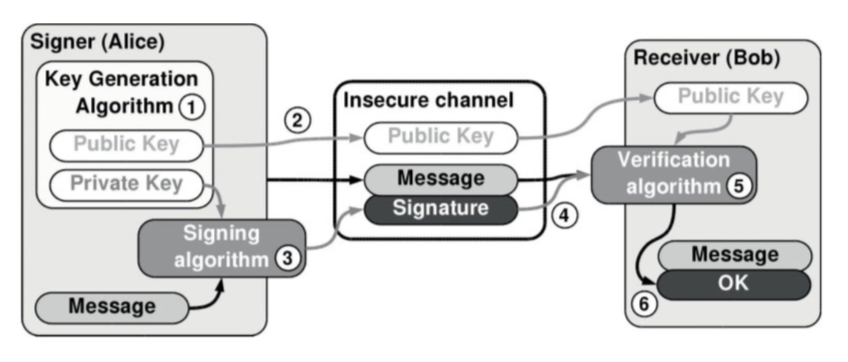
\includegraphics[width=8cm]{images/10.png}
    \caption{Digital signature system}
\end{figure}

\noindent First, the signer (Alice) generates a public– private keypair, using the key generation algorithm (1). She sends her public key through the communication channel (2). Next, Alice uses the private key to digitally sign the message (3). It is important that she keeps the private key to herself, not revealing it to anyone. Once the message has been signed, both the message and the signature are sent to the receiver (Bob) (4). Note that the message is not encrypted, but only authenticated. Bob verifies the signature, using Alice’s public key (5). If the verification yields a positive result, he knows that the message was originated by Alice (6). Otherwise, he can reject the message as invalid.\newline
A technical point with digital signatures is that the message could be of an arbitrary length. This can be a problem because the algorithms employed by public key cryptography are quite slow. The solution to this problem is to first take the hash8 of the (arbitrarily long) message, and then sign this hash. The output of a hash function is of the same (shorter) length, independent of the size of the input. Using this hashing step, messages of arbitrary length can be signed explicitly.\newline
A digital signature protocol is the combination of a public-key algorithm with a digital signature scheme. The public-key algorithm provides the underlying asymmetric mathematical algorithm. The digital signature scheme proposes a way to use this asymmetric algorithm to arrive at a workable digital signature. There are three main public key families used in practice:
\begin{itemize}
    \item Integer factorization. These algorithms are based on the difficulty of factoring large integers;
    \item Discrete logarithm (DL). Based on the intractability of the discrete logarithm problem on finite cyclic groups;
    \item Elliptic curve (EC). Based on the difficulty of computing the generalized logarithm problem on an elliptic curve.
\end{itemize}
The main digital signature schemes used in practice are:
\begin{itemize}
    \item RSA. The RSA signature scheme is based on the RSA algorithm. It is the most widely used digital signature scheme;
    \item Schnorr signature. It is considered the simplest signature scheme that can be used both with discrete logarithm and elliptic curve algorithms. This results in small computational times for signing and verification, as well as smaller signatures.
    \item DSA. It stands for Digital Signature Algorithm and was proposed by NIST in 1991 (Wikipedia, 2014). This scheme is widely used, in part because the patent that covers it was made available worldwide royalty-free.
\end{itemize}

\subsection*{Elliptic Curves}
The elliptic curve protocol starts from a given known point, called the generator. A public key is a point in the elliptic curve. A private key is the number of steps from the generator that must be traversed to arrive at the public key point. Computing the public key given the private key is very fast, thanks to the double-and-multiply algorithm. But the reverse, given the public key finding out the private key, is very difficult. This is known as the discrete logarithm problem. The brute-force algorithm to solve the discrete logarithm problem would traverse the points in the elliptic curve one at a time starting from the generator until it arrives at the desired point. Fortunately this algorithm is computationally infeasible, taking a ridiculous number of years to complete with classical computers.\newline
Given the generator of the curve \textit{A} and a private key \textit{d}, it is fast to compute the public key \textit{P = d \(\cdot\) A}, but the reverse, given \textit{A} and \textit{P} compute \textit{d}, is infeasible with current computers. Any number of messages can be signed if in possession of the private key \textit{d}. To sign each of these messages a nonce, a random number used only once per private key, must be generated. It is very important that this nonce is never reused. Reusing it just once gives away the private key \textit{d} and thus the funds in a Bitcoin address. Symmetric ciphers are more efficient for the same level of security than public key ciphers, both in terms of speed and key sizes. Furthermore, modern symmetric ciphers such as AES are resistant to quantum computing. But as explained at the beginning of the chapter, symmetric ciphers cannot be used for digital signing schemas. The following picture shows the key sizes required to obtain a certain security level for various public key cryptography algorithms: RSA, discrete logarithm (DL), and Elliptic Curve Cryptography (ECC). The security level is defined as the key length of a symmetric systems, such as AE, with the same security.

\begin{figure}[H]
    \centering
    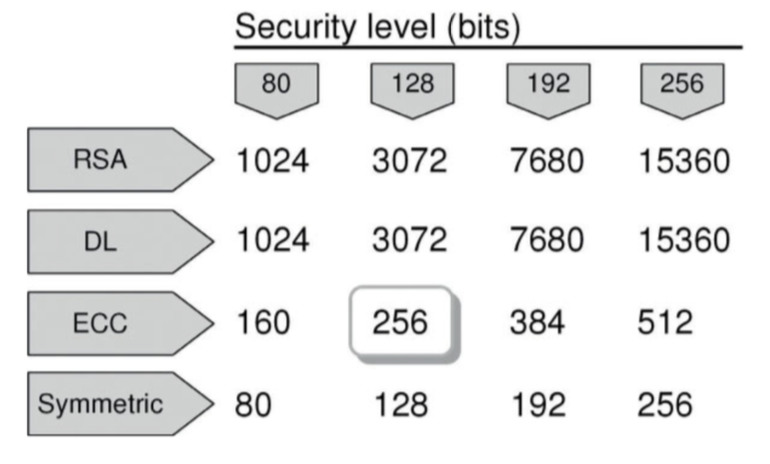
\includegraphics[width=8cm]{images/11.png}
    \captionsetup{width=.8\linewidth}
    \caption{Key size of several public key cryptography algorithms to obtain various security levels}
\end{figure}

\noindent Thus, as the bottom row shows, the key length of a symmetrical cipher coincides with the security level. It should be clear why Satoshi chose ECC: 256-bit elliptic curve digital signatures provide the smallest key sizes for a given level of security, 128 bits in Bitcoin’s case. Size is an important factor in Bitcoin, because a large portion of the data that is stored in the blockchain are the ECC signatures for the transactions. If Bitcoin were to use RSA, the size of the signatures would increase by a factor of 12.\newline
The curve used in Bitcoin is called \textit{secp256k1}, whose points verify the equation:
\[ y^2 = x^3 + ax + b \]
where \(a = 0\) and \(b = 7\).
\textit{Secp256k1} was already never used before Bitcoin’s became popular, but it is now gaining in popularity due to its several property. It was constructed in a special non-random way which allow for especially efficient computation. As a result it is often more than 30\% faster than other curves if the implementation is sufficiently optimized. \textit{Secp256k1}’s constant were selected in a predictable way in order to avoid any sort of backdoor in custom elliptic curves. Currently Bitcoin uses \textit{secp256k1} with the ECDSA algorithm (Elliptic Curve Digital Signature Algorithm). ECDSA ensure that Bitcoins can only be spent by their rightful owner.\newline
As excerpted from standard, the elliptic curve domain parameters over \(\mathbb{F}_{p}\) associated with a \textit{Kobraliz} curve, \textit{secp256k1} are specified by the sextuple \(T = (p, a, b, G, n, h)\) where the finite field \(\mathbb{F}_{p}\) is defined by:
\begin{itemize}
    \item \(p\) is the order of the finite field. \begin{dgroup*}\begin{dmath*}p = F^8F^8F^8F^8F^8F^8FFFFFFFEFFFFFC2F = 2^{256} -2^{32} -2^9 -2^8 -2^7 -2^6 -2^4 -1\end{dmath*}\end{dgroup*}
    \item The elliptic curve \(E:y^2 =x^3+ax+b\) is defined by \(a = 0\) and \(b = 7\).
    \item \(G\) is the base point. In a compressed form is equal to:\par\noindent \(G = \seqsplit{0279BE667EF9DCBBAC55A06295CE870B07029BFCDB2DCE28D959F2815B16F81798}\)
    \item The order \(n\) of \(G\):\par\noindent
    \(p = F^8F^8F^8F^8F^8F^8\seqsplit{FFFFFFFEBAAEDCE6AF48A03BBFD25E8CD0364141}\)
    \item \(h\) is the cofactor and is equal to 1
\end{itemize}
\textit{Secp256k1} has characteristic \(p\), it is defined over the prime field \(\mathbb{Z}_{p}\). In cryptography, an elliptic curve is a group with given size \(k\). Normally we use a subgroup of prime order \(r\), where \(r\) divides \(k\). The “cofactor” is \(h = k/r\). For every point \(P\) on the curve, the point \(hP\) is either the “point at infinity”, or it has order \(r\); i.e., when taking a point, multiplying it by the cofactor necessary yields a point in the subgroup of prime order \(r\).\newline
When the cofactor is equal to 1, we will refer to the whole curve (as in the case of \textit{secp256k1}). Any incoming point \((x,y)\) that fulfills the curve equation is part of the curve. When the cofactor is different from 1, then the subgroup of prime order is a strict subset of the curve. When we are considering a point and verifying that it is on the curve, it is not sufficient to guarantee that the point belong to the subgroup that we are considering. Moreover, there will be points that order is not a multiple of \(r\).\newline
Since \textit{secp256k1} is based on Kobraliz curve a particular feature is that the computation of point multiplication is much more faster than calculate the resulting point in the elliptic curve. This feature is based on the Frobenius map.

\paragraph*{Frobenius map:}
In commutative algebra and field theory, the Frobenius endomorphism (after Ferdinand Georg Frobenius) is a special endomorphism of commutative rings with prime characteristic \(p\), an important class which includes finite fields.\newline
Let \(E\) be an elliptic curve given by a generalized Weierstrass equation, whose coefficients are among numbers \(0, 1, ..., p - 1\), i.e., elements of \(\mathbb{Z}_{p^k}\). The points of \(E\) are taken with coordinates in \(\mathbb{Z}_{p^k}\) which gain in efficiency in our algorithms. A key tool in the study of elliptic curves is the Frobenius automorphism \(\tau : \mathbb{Z}_{p^k} \rightarrow \mathbb{Z}_{p^k}\) defined by the simple rule:

\[\tau x = x^p;\hspace{0.5cm}\tau(x+y) = \tau x+\tau y;\hspace{0.5cm}\tau(x \cdot y) =  \tau x \cdot \tau y\]

\noindent We extend the Frobenius map on point \(P = (x, y) \in E(\mathbb{Z}_{p^k})\) by applying \(\tau\) to each coordinate:

\[\tau(P) = (\tau x,\tau y)\]

\noindent We can say that:
\begin{itemize}
    \item \(\tau(P) \in E(\mathbb{Z}_{p^k})\)
    \item \(\tau E(\mathbb{Z}_{p^k}) \rightarrow E(\mathbb{Z}_{p^k})\) is a group endomorphism:\[\tau(P + Q) = \tau(P) + \tau(Q) \hspace{0.5cm}\forall P,Q \in E(\mathbb{Z}_{p^k})\]
\end{itemize}

\noindent Let \(E : y^2 + a_1xy + a_3y = x^3+ a_2x^2 + a_4x + a_6\) be a generalized Weierstrass elliptic curve over \(\mathbb{Z}_{p}\) and let:
\[t = p + 1 - E(\mathbb{Z}_{p})\]
by Hasse’s theorem \(|t| \leq \sqrt{4p}\), i.e., \(t^2 \leq 4p\).\newline
Let \(\alpha\) and \(\beta\) be the conjugate complex roots of the quadratic polynomial:\newline
\[z^2 - tz + p = 0; \hspace{0.5cm} \alpha,\beta = (t \pm \sqrt{t^2 - 4p})/2,(t^2 - 4p < 0)\]
The \(\mid	\alpha \mid\) = \(\mid	\beta \mid\) = \(\sqrt{4p}\), and \(\forall k \geq 1\) we have
\[E(\mathbb{F}_{p^k}) = p^k + 1 - \alpha^k - \beta^k\]
Let
\[\tau : E(\mathbb{F}_{p^k} \rightarrow E(\mathbb{F}_{p^k})); \hspace{0.5cm} (x,y) \rightarrow (x^p , y^p) \]
be the Frobenius map. Then, for every point \(Q = (x, y) \in E(\mathbb{F}_{p^k})\),
\[\mathcal{O} = \tau^2(Q) - t\tau(Q) + pQ = (x^{p^2} , y^{p^2} ) + t(x^p, - y^p - a_1x^p - a_3) + pQ\]

\paragraph*{Koblitz curve:} is an elliptic curve defined over \(\mathbb{F}_{2}\) by an equation of the form
\[E_a : y^2 + xy = x^3 + ax^2 + 1, a \in \{0,1\}\]
\textit{Secp256k1} belongs to Koblitz’s curve cryptosystem. The Koblitz’s idea was to replace the multiplication by 2 map with the Frobenius map \(\tau\). If \(P = (x, y)\) it takes much less time to compute \(\tau(P) = (x^2, y^2)\) that computing \(P + P\) in the elliptic curve.\newline
With these formalities out of the way, we are now in a position to understand private and public keys and how they are related. Here it is in a nutshell: In ECDSA, the private key is an unpredictably chosen number between 1 and the order. The public key is derived from the private key by scalar multiplication of the base point a number of times equal to the value of the private key. Expressed as an equation:\newline\newline
\centerline{public key = private key \(\cdot\) base point}\newline\newline
This shows that the maximum possible number of private keys (and thus Bitcoin addresses) is equal to the order.\par
\noindent In a continuous field we could plot the tangent line and pinpoint the public key on the graph, but there are some equations that accomplish the same thing in the context of finite fields. Point addition of \(p + q\) to find \(r\) is defined component-wise as follows:
\[c = (q_y - p_y)/(q_x - p_x)\]
\[r_x = c^2 - p_x - q_x\]
\[r_y = c(p_x - r_x) - p_y\]
And point doubling of \(p\) to find \(r\) is as follows:
\[c = (3p_{x^2} )/(2p_y)\]
\[r_x = c^2 - 2p_x\]
\[r_y = c(p_x - r_x) - p_y\]

\noindent In practice, computation of the public key is broken down into a number of point doubling and point addition operations starting from the base point.\newline
Let’s run a back of the envelope example using small numbers, to get an intuition about how the keys are constructed and used in signing and verifying. The parameters we will use are:
\begin{itemize}
    \item Equation: \(y^2 = x^3 + 7\);
    \item Prime modulo: \(67\);
    \item Base point: \((2, 22)\);
    \item Order : \(79\);
    \item Private key: 2.
\end{itemize}
First, let’s find the public key. Since we have selected the simplest possible private key with \(value = 2\), it will require only a single point doubling operation from the base point. The calculation looks like this:
\[c = (3 \cdot 2^2 + 0)/(2 \cdot 22) \bmod 67\]
\[c = (3 \cdot 4)/(44) \bmod 67\]
\[c = 12/44 \bmod 67\]
Here we have to pause for a bit of sleight-of-hand: how do we perform division in the context of a finite field, where the result must always be an integer? We have to multiply by the inverse, which space does not permit us to define here. In the case at hand, you will have to trust us for the moment that:
\[44^{-1} = 32\]
Moving right along:
\[c = 12 \cdot 32 \bmod 67\] 
\[c = 384 \bmod 67\]
\[c = 49\]
\newline
\[r_x = (49^2 - 2 \cdot 2) \bmod 67\]
\[r_x = 2397 \bmod 67\]
\[r_x = 52\]
\newline
\[r_y =(49 \cdot (2 - 52) - 22) \bmod 67\]
\[r_y =(49 \cdot (-50) - 22) \bmod 67\]
\[r_y = (-2450 - 22) \bmod 67\]
\[r_y = -2472 \bmod 67\]
\[r_y = 7\]
Our public key thus corresponds to the point \((52, 7)\). All that works for a private key of \(2\)!\newline
This operation - going from private to public key - is computationally easy in comparison to trying to work backwards to deduce the private key from the public key, which is theoretically possible but computationally infeasible due to the large parameters used in actual elliptic cryptography.\newline
Therefore, going from the private key to the public key is by design a one-way trip.\newline
As with the private key, the public key is normally represented by a hexadecimal string. But wait, how do we get from a point on a plane, described by two numbers, to a single number? In an uncompressed public key the two 256-bit numbers representing the \(x\) and \(y\) coordinates are just stuck together in one long string. We can also take advantage of the symmetry of the elliptic curve to produce a compressed public key, by keeping just the \(x\) value and noting which half of the curve the point is on. From this partial information we can recover both coordinates.

\subsection*{Signing data with the private key}
Now we will show how to sign data with the private key.\newline
The data can be of any length. The usual first step is to hash the data to generate a string containing the same number of bits (256) as the order of the curve. Here, for the sake of simplicity, we’ll skip the hashing step and just sign the raw data \(z\). We’ll call \(G\) the base point, \(n\) the order, and \(d\) the private key. The recipe for signing is as follows:
\begin{itemize}
    \item Choose some integer \(k\) between \(1\) and \(n - 1\);
    \item Calculate the point \((x,y) = k \cdot G\), using scalar multiplication or Frobenius map in case of Koblitz’s curve (secp256k1);
    \item Find \(r = x \bmod n\). If \(r = 0\), return to step 1;
    \item Find \(s = ( z + r \cdot d)/k \bmod n\). If \(s = 0\), return to step 1;
    \item The signature is the pair \((r, s)\).
\end{itemize}

\subsubsection*{Example:}\par\noindent
\begin{adjustwidth}{2.5em}{0pt}
    \(z = 17\) (data)\newline
    \((r, s) = (62, 47)\) (signature)\newline
    \(n = 79\) (order)\newline
    \(G = (2, 22)\) (base point)\newline
    \(Q = (52, 7)\) (public key)
\end{adjustwidth}
Verify that \(r\) and \(s\) are between \(1\) and \(n – 1\) : 
\begin{adjustwidth}{2.5em}{0pt}
    \(r: 1 \leq 62 < 79\)\newline
    \(s: 1 \leq 47 < 79\)
\end{adjustwidth}
Calculate \(w\):
\begin{adjustwidth}{2.5em}{0pt}
    \(w = s - 1 \bmod n\)\newline
    \(w = 47 - 1 \bmod 79\)\newline
    \(w = 37\)
\end{adjustwidth}
Calculate \(u\):
\begin{adjustwidth}{2.5em}{0pt}
    \(u = zw \bmod n\)\newline
    \(u = 17 \cdot 37 \bmod 79\)\newline
    \(u = 629 \bmod 79\)\newline
    \(u = 76\)
\end{adjustwidth}
Calculate \(v\):
\begin{adjustwidth}{2.5em}{0pt}
    \(v = rw \bmod n\)\newline
    \(v = 62 \cdot 37 \bmod 79\)\newline
    \(v = 2294 \bmod 79 \)\newline
    \(v=3\)
\end{adjustwidth}
Calculate the point \((x, y)\):
\begin{adjustwidth}{2.5em}{0pt}
    \((x, y) = uG + vQ\)
\end{adjustwidth}
Let’s break down the point doubling and addition in \(uG\) and \(vQ\) separately.
\begin{adjustwidth}{2.5em}{0pt}
    \(uG = 76G \newline
    uG = 2(38G) \newline
    uG = 2( 2(19G) ) \newline
    uG = 2( 2(G + 18G) ) \newline
    uG = 2( 2(G + 2(9G) ) ) \newline
    uG = 2( 2(G + 2(G + 8G) ) ) \newline
    uG = 2( 2(G + 2(G + 2(4G) ) ) ) \newline
    uG = 2( 2(G + 2(G + 2( 2(2G) ) ) ) ) \)
\end{adjustwidth}
We reduce by grouping \(75\) successive addition operations to just six operations of point doubling and two operations of point addition. These tricks will come in handy when the numbers get really large.\newline
Working our way from the inside out:
\begin{adjustwidth}{2.5em}{0pt}
    \(uG = 2( 2(G + 2(G + 2( 2( 2(2, 22) ) ) ) ) ) \newline
    uG = 2( 2(G + 2(G + 2( 2(52, 7) ) ) ) ) \newline
    uG = 2( 2(G + 2(G + 2(25, 17) ) ) ) \newline
    uG = 2( 2(G + 2( (2, 22) + (21, 42) ) ) ) \newline
    uG = 2( 2(G + 2(13, 44) ) ) \newline
    uG = 2( 2( (2, 22) + (66, 26) ) ) \newline
    uG = 2( 2(38, 26) ) \newline
    uG = 2(27, 40) \newline
    uG = (62, 4) \)
\end{adjustwidth}
And now for \(vQ\):
\begin{adjustwidth}{2.5em}{0pt}
    \(vQ = 3Q \newline
    vQ = Q + 2Q \newline
    vQ = Q + 2(52, 7) \newline
    vQ = (52, 7) + (25, 17) \newline
    vQ = (11, 20)\) 
\end{adjustwidth}
\break
Putting them together:
\begin{adjustwidth}{2.5em}{0pt}
    \((x, y) = uG + vQ \newline
    (x, y) = (62, 4) + (11, 20) \newline
    (x, y) = (62, 63)\)
\end{adjustwidth}
Clearly step 5 is the bulk of the work. For the final step verify that \(r = x \bmod n\):
\begin{adjustwidth}{2.5em}{0pt}
    \(r = x \bmod n \newline
    62 = 62 \bmod 79 \newline
    62 = 62\)
\end{adjustwidth}
Our signature is valid!

\subsection*{Hash Functions}
A hash function is an algorithm that takes data of arbitrary length as an input and outputs a bit-string of fixed length, named the hash value. The hash value is always the same for the same input data. A hash function is a map from the set of input data (of arbitrary length) to the set of hash values, with the particularity that small differences in the input data produce large differences in the result. A common requirement is that hash computation is fast. Bitcoin uses cryptographic hash functions to perform proof-of-work. Cryptographic hash functions impose additional requirements over regular hash functions:
\begin{itemize}
    \item One-wayness (preimage resistance). Given the hash value, it must be computationally infeasible to find out the input data;
    \item Weak collision resistance. Given an input it is computationally infeasible to find another input with the same hash value;
    \item Strong collision resistance. It is computationally infeasible to find two input data points that result in the same hash value.
\end{itemize}
Bitcoins uses SHA256 as its proof-of-work function. SHA256 meets the preimage resistance requirement: given the hash value it is computationally infeasible to recover the message that generated it. Computationally infeasible means that there is no known algorithm that can recover the message within a time that is related polynomially to the size of the input. This means, in practice, that the best known algorithm to break hashing function are the brute-force algorithm that take an exponential time to recover the original message.

\subsection*{Proof-of-Work}
Now we are going to briefly resume the concept of proof-of-work previously described and analyzed it in more details.\par\noindent
The proof-of-work could be the solution of a computationally-hard problem, a memory-hard problem, a problem requiring user intervention, and so on. The problem must be moderately hard to solve but easy (computationally fast) to verify. A service provider can then pose the problem to anyone who requests the service, and only grant access to those users that pass the challenge. Proof-of-work systems can be implemented following two protocols:
\begin{itemize}
    \item Challenge-Response. This protocol assumes an ongoing communication between the client and the server. First the client requests the service, then the server chooses a proof-of-work and challenges the client. The client then has to solve the proof-of-work and send the response to the server. Finally the server verifies that the proof-of-work has been correctly done and then grants the client access to the service;
    \item Solution-Verification. This protocol is asynchronous: solution and verification can be done at different times. Ongoing communication between the server and the client is not required. First, the client creates a proof-of-work problem and solves it. This problem should be different every time and chosen by an algorithm, for instance, the client could use the result of a hash function to generate it. Then the client sends the solution to the server, who verifies it and proceeds accordingly.
\end{itemize}
To secure the blockchain, Bitcoin requires proof-of-work to be performed on blocks of transactions following the Solution-Verification protocol. Bitcoin uses partial hash inversion as the proof-of-work function. Partial hash inversion requires that the hash of a block of transactions matches a certain pattern. The pattern to match is that the hash starts with at least a certain number of 0 bits.
\par\noindent The blockchain is an ever-growing chain of blocks. Each block contains a group of new transactions and a link to the previous block in the chain. New transactions in the network are collected into a block which is appended to the blockchain.\newline
Each block is secured with a partial hash inversion proof-of-work. First, each block includes a group of (valid) transactions, the hash of the previous block, and a nonce. The nonce in a block solves the partial hash inversion problem. That is, the nonce is a number such that the hash of the entire block (including the nonce) starts with a certain number of zero bits.\newline
The persons or institutions contributing their computational power to solve the proof-of-work are called miners. The assistance of the miners is critical to secure the blockchain, and the protocol compensates them with newly minted Bitcoins (block reward).\newline
Every block includes a special transaction called the coinbase. The coinbase is the first transaction in a block. It has only one transaction input (TxIn), which is not linked to any previous transaction output (TxOut) and does not serve any purpose. On the other hand, the coinbase can have many outputs. The sum of values in these outputs are equals to the block reward, plus the sum of all the fees granted by the transactions collected into the block. Miners can choose which transactions to include in the blocks they mine, and they usually decide to include them based on the fee they pay. The miner who solves the hashing problem uses the coinbase to pay the block reward to itself. This is why solving the partial hash inversion problem is called mining. All miners in the network compete to mine blocks. The hash rate of a miner is its computational power, measured in hashes/second (hash per second). The network hash rate is the total hash rate of all the miners in the network, and it stands at around 30,000 TH/s at the time of writing.\newline
The block preceding a given block is called its parent block. Blocks reference their parent block in the blockchain by including its hash in their data structure. Thus the blockchain keeps blocks in chronological order. The first block in the blockchain is called the genesis block and it was created by Satoshi in January 3, 2009.\newline
The order of a block in the blockchain, starting from the genesis block is called the block height. The last block added to the blockchain is called the blockchain head. New blocks are added on top of the blockchain head.\newline
A fork occurs when two miners arrive at a new block at roughly the same time. Both blocks solve the partial hash inversion problem, but only one of them can be part of the long-term blockchain. The discarded block is called an orphan block.\newline
The decision of which branch of the blockchain is the valid one is not taken by any party. Transactions included in the blocks of a fork are not lost. When a fork is resolved and a branch of the blockchain is discarded, the transactions in that branch are introduced again into the unconfirmed transactions’ memory pool, ready to be included in the next block mined. Every fork resolution produces winners (the miners that solved blocks in the accepted branch) and losers (miners whose solved orphaned blocks). The Bitcoin protocol solves a fork in favor of the longest blockchain. Blockchain length is measured by the combined difficulty of all the blocks in the chain.\newline
The Bitcoin network is composed of nodes. Nodes are computers connected to the internet, running the Bitcoin software. The Bitcoin network is a peer-to-peer network: all nodes are homogeneous. Nodes receive transactions and blocks from other nodes, and relay these transactions and blocks to other nodes. Each node keeps a full copy of the blockchain.\newline
A newly created transaction that has not been included into any block is called an unconfirmed transaction. Once a transaction is included in a block it is said to be confirmed. When a miner finds a new block, it broadcasts it to the network. All receiving nodes first check the validity of the block. They then update their internal data structures to reflect the new information contained in the block.

\subsection*{Double Spending and 51\% Attack}
A double-spend attempt occurs when two different transactions try to spend the same funds. The Bitcoin protocol defends against this attack by deciding that the valid transaction is the one that finds its way into the blockchain first. Thus Bitcoin solves the double-spending problem in a decentralized way, without the need for a central authority to decide which transaction is valid. An attacker wishing to change the blockchain at a certain block would have to mine again all blocks from that block up to the blockchain head. Moreover, as the Bitcoin network keeps on adding blocks to the blockchain, the attacker would not only have to redo all the past work, but would have to keep up with the pace of new legitimate block creation and surpass it. The only way an attacker could perform such a feat is to command a hash rate as large as the hash rate of the rest of the network, this attack is called a 51\% attack.

\subsection*{Scalability}
There is a limit to the maximum block size hard-coded into Bitcoin Core. This limit is currently set at 1 MB. This limit could be increased in future versions of Bitcoin Core if and when the tps (transaction per second) of the Bitcoin network increases. The bottlenecks that could prevent Bitcoin scaling to match the rates of established payment processing networks can be divided in three groups:
\begin{itemize}
    \item Computational power. Nodes perform two main computing tasks: checking block hashes and checking transaction signatures. A current single core is able to process 8,000 ECDSA signatures/second. Therefore a single core machine could process 4,000 tps. As signature checking is a highly parallelizable task, adding more cores can further increase the tps a machine could handle;
    \item Network. Transactions currently average 0.5 kB in size. Again, this average will probably increase in the future with the increased importance of multi-signature transactions;
    \item Storage. As transactions take on average 0.5 kB of storage, storage utilization could quickly escalate for high transaction rates. For instance, a rate of 2,000 tps generates around 1 MB of data every second, or 30 TB of data every year. Furthermore, with the increased utilization comes an increase in the number of unspent transaction outputs, thus increasing the RAM memory requirements for the UTXO, probably making impossible for the UTXO to fit in RAM.
\end{itemize}
For the time being, with the current value of the maximum block size set at roughly 1MB there is ample room to collect all the new transactions in the network: this block size could accommodate 3 to 4 tps. As the number of transactions increases, this value could be increased accordingly.

\subsection*{Wallets}
As we already said earlier, Bitcoins are saved as an entry into a distributed ledger, the blockchain. The private key associated with an address must be used to sign a transaction spending the funds from that address. A Bitcoin wallet is simply a collection of private keys. The main features of a Bitcoin wallet are:
\begin{itemize}
    \item A Bitcoin wallet can be copied, this means that whoever controls a copy of the Bitcoin wallet (knows the private key) can spend the funds;
    \item A Bitcoin wallet can be distributed across several devices, in such a way that accessing the funds might require cooperation between the devices;
    \item There’s also a ’receive-only’ Bitcoin type of wallet. This type of wallet can receive funds but cannot spend funds from their addresses.
\end{itemize}
A wallet software is a piece of software that allows spending funds from the addresses in a wallet and to manage the wallet. The tasks performed by the wallet software usually include:
\begin{itemize}
    \item Query the blockchain and present to the user a total of the funds available;
    \item Generate new addresses to receive new funds;
    \item Interface with the user, for instance generating or reading QR codes
representing addresses, transactions, etc.;
    \item Allow the user to send funds to addresses of his/her choices;
    \item Track transactions’ confirmation status;
    \item Make a backup of the wallet;
    \item Restore a backup of the wallet.
\end{itemize}
A Bitcoin address is like a bank account. The Bitcoin equivalent of opening an account is downloading wallet software and letting the software generate a private-public key pair. This key pair, as we saw in the previous chapters, must be difficult to guess in order to avoid thefts by some attackers and so to steal the founds from the wallet. To secure against this attack, the wallet software must generate private keys with a high degree of entropy. One way to achieve this is to use a good (pseudo)random number generator. This is the approach followed by many wallet software implementations.\newline
In an address tampering attack, a user is misled into sending funds to an incorrect address. An address tampering attack takes places when a user is about to send funds to an address and an attacker intercepts the legitimate address and substitutes it by an address under its control. An attacker that achieves man-in-the-middle status could easily change the receiving address in a payment.\newline
Finally, to guard against a loss of key a user should back up the wallet quite often.\par\noindent 
\textbf{Offline wallets:} Usually the device that holds a wallet is connected to the internet, in order to communicate with the Bitcoin network (receiving account status, sending transactions, observing confirmations, and so on). This is called an online wallet or a hot wallet. As every device connected to the internet is at risk of being compromised, it is good practice to hold the funds in a offline wallets, whose private keys are not accessible from the internet. Note that an offline wallet can sign transactions offline. Cold storage refers to a place where the private keys are kept, that is not accessible from the internet.\par\noindent
\textbf{External storage media:} One way to create cold storage for the private keys is to save them in external storage media, such as USB flash drives or optical disks. Only when a private key it needed, such as when signing a transaction, is retrieved from the external storage.\newline
If the private keys are retrieved by an online wallet, the device with the online wallet could be compromised and the file with the private keys stolen by an attacker. Therefore it is advisable to encrypt the file holding the private keys when saved in external media.\newline
In summary, when using external storage, the weak link is the period where the private keys are imported to the online client to sign transactions. It is more secure to import the private keys from cold storage to an offline wallet.\par\noindent
\textbf{Paper wallets:} Another way to create cold storage for the private keys is to print them on a piece of paper and to protect that piece of paper from physical theft. These are called paper wallets, although they are not technically a wallet. In a paper wallet, public keys or Bitcoin addresses are usually printed alongside the private keys, so that the paper wallet can be easily identified without having to import the private key into a client.\newline
As a good security practices it is recommended that paper wallets are generated using offline devices, i.e. a computer connected to a printer, with both of them offline. The devices should be rebooted before and after generating the paper wallet to avoid leaving sensitive information in the devices’ memory. It is advisable that the device generating the paper wallet is booted from a live CD to avoid spyware stealing the private keys.\newline
As was the case for external storage, the private keys from the paper wallet must be imported into the wallet software to be able to sign transactions. If the paper wallet is imported to an online wallet, the keys are at risk of being seized by any malware that the device could be running. Thus paper wallets should only be imported moments before the funds will be used.\par\noindent
\textbf{Web wallets:} Web wallets are online accounts where a user can deposit its funds. The funds are controlled by the web wallet provider. By authenticating with the web wallet provider, the user can later access those funds, i.e. make transactions. The main advantage of web wallets are that they are easy to set up and to use it, but note that, in addition to the risk of the web wallet provider stealing their users’s funds (e.g. Mt. Gox case), there is the risk that the provider is hacked and loses the funds, thus making the service insolvent.\par\noindent
\textbf{Brain wallets:} Brain wallets generate a private key by hashing a long password or passphrase (e.g. using the SHA256, since the Bitcoin private keys are 256 bits long). A brain wallet’s password does not need to be stored in a device; rather it should be stored in the brain of the user - hence the name. Brain wallets have a big disadvantage that should dissuade anyone from using them: they are subject to brute-force attacks that could steal all the funds in the wallet if successful. The chances of success of these attacks are very high. First, users are very bad at choosing passwords with a high degree of entropy. Second, password cracking technology has got much better in the last years, thanks to technologies such as dictionary attacks, rainbow tables, GPUs and the fact that several big password databases have been leaked.\par\noindent
\textbf{Deterministic wallets:} A deterministic wallet is a wallet that can generate many addresses (and their associated private keys) from a common private key.

\begin{figure}[H]
    \centering
    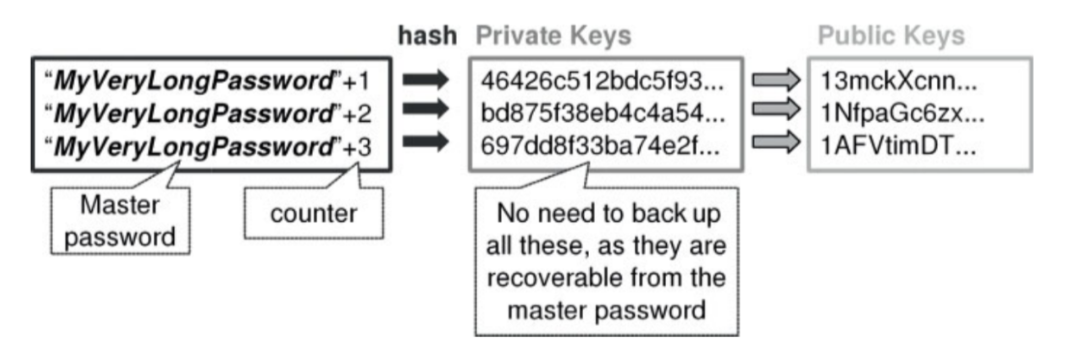
\includegraphics[width=12cm]{images/12.png}
    \caption{Deterministic wallets}
\end{figure}

\noindent There are two type of deterministic wallet:
\begin{itemize}
    \item \textbf{Type-1 deterministic}: The addresses generated by this type are impossible to relate to one another by anyone who does not know the master password (problem: susceptible to brute-force attacks);
    \item \textbf{Type-2 deterministic}: Allows the separation of the roles of generating a private key and generating an address. These wallets use the properties of elliptic curves to calculate new public keys without revealing private keys.
\end{itemize}
\textbf{Hierarchical deterministic wallets:} Hierarchical Deterministic wallets (HD wallets) are deterministic wallets whose derived addresses form a hierarchy. As with deterministic wallets, all their addresses can be derived from a starting secret. The novelty introduced by HD wallets is that the addresses it generates are sorted in a tree structure such that a node has visibility of its descendants but not of its ascendants. There are two types of nodes in the tree: private nodes that hold the private keys to the sub-tree originating from them, and public nodes that hold only the public keys to their sub-tree. Aside from the private and public keys, each node has an additional field called the ‘chain code’. The goal of the chain code is to add additional entropy to each node. Thus revealing an address does not automatically reveal the tree derived from that node.

\begin{figure}[H]
    \centering
    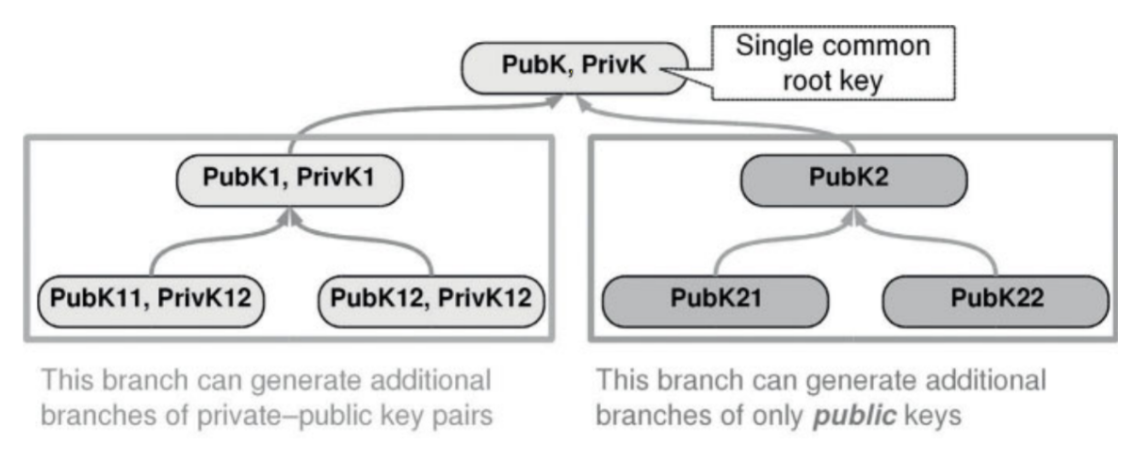
\includegraphics[width=12cm]{images/13.png}
    \caption{Hierarchical deterministic wallets}
\end{figure}

\subsubsection*{Simplified Payment Verification (SPV)}
Full Bitcoin nodes verify new blocks that are added to the blockchain by checking that all transactions included are properly signed and that the hash of the blocks satisfy the proof-of-work difficulty. During this process, full nodes maintain a cache of unspent transaction outputs that they can be queried by a wallet to determine the amount of funds available in the addresses controlled by that wallet. A wallet implementation following this approach has two disadvantages that make it unpractical for lightweight clients:
\begin{itemize}
    \item It requires downloading and storing the full blockchain;
    \item It requires a full node verifying all blocks and all transactions contained in those blocks (the verification process uses a lot of energy - not possible using a mobile device).
\end{itemize}
One possible solution would be to run a wallet client that would connect to a trusted server. The wallet would use the trusted server as a proxy to connect to the Bitcoin network. It could query the server for new transactions to certain addresses periodically, and it could use the server to relay signed transactions to the network.\newline
Another possible solution is to use a Simplified Payment Verification (SPV) wallet. An SPV client only keeps a copy of the block headers. When an SPV client needs to verify a transaction it downloads the Merkle branch that binds the transaction to the block header.\par\noindent
When there are conflicting branches, i.e. a fork in the blockchain, a regular node will assume the longest blockchain (in terms of difficulty) is the legitimate one. Thus a regular node determines the validity of transactions by their inclusion in a block that belongs to the longest chain. This is called the ‘block height’ validity check. In contrast, an SPV client determines the validity of a transaction by how many blocks have been mined on top of the block where the transaction is included. This is called the ‘block depth’ validity check.

\subsection*{Mining}
As mentioned in the previous sections, mining Bitcoin is the process of adding new blocks to the blockchain. Miners contribute using their computational power to solve the blocks that are added to the blockchain, and the network remunerates them with the block reward and the fees collected from all the transactions included in the block. Bitcoin is a peer-to-peer network; anyone can connect to it and start mining right away. To find a solution, mining software usually increments the block nonce and runs the proof-of-work algorithm to check if the chosen nonce generates a correct block hash (i.e. a block hash that meets the difficulty requirements). One of the advantages of the mining mechanism is that it rewards early adopters for supporting the network. This was very important in the beginning, when Bitcoin bootstrapped itself into relevance. Bitcoin does not have a corporation backing it, so marketing had to be done virally.\newline
The mining difficulty increases as more miners enter the network, but the total block reward stays the same. The block reward is halved every 210,000 blocks (roughly every 4 years).

\subsection*{Mining Technology}
The network hash rate has had an exponential growth due to two trends:
\begin{itemize}
    \item Exponential growth in the price of Bitcoin itself, which has attracted a lot of mining investment;
    \item Advances in mining technology (new hardware to mine Bitcoin).
\end{itemize}
Mining hardware has followed a trend toward more specialized hardware where a larger part of the circuitry of the chip is dedicated to the hashing function. There have been four phases in this transition:
\begin{itemize}
    \item \textbf{CPUs}: It is a general purpose hardware. Its computational power can be applied to many tasks, including mining Bitcoin. During the first phase of Bitcoin mining, running from 2009 to the summer of 2010, mining was performed only using CPUs. For comparisons the latest retail processors offer a hash rate of approximately 20MH/s.
    \item \textbf{GPUs}: Hardware originally used for graphic acceleration. There is a trend in computing of using the parallel power of GPUs to perform general computations. Starting in mid-2010, GPUs were programmed to mine Bitcoins, quickly rendering CPU mining uneconomical. GPUs offer an advantage over CPUs because they are composed of hundreds or even thousands of computational units, compared with the handful in a typical CPU. For comparison the latest GPUs offer a hash rate ranging from 100MH/s to 500MH/s.
    \item \textbf{FPGAs (Field-Programmable Gate Array)}: They are chips built of logic blocks that can be programmed and interconnected to perform a particular task. FPGAs were introduced in Bitcoin mining in mid-2011 and for a time competed with GPUs. GPUs held the advantage on cost per GH/s and resale value, while FPGAs had an advantage in lower power consumption. Typical FPGAs have a hash rate of approximately 1 GH/s.
    \item \textbf{ASICs (Application-Specific Integrated Circuit)}: They are chips built for a specific application, in contrast to CPUs that accept software running many possible applications. ASIC parts have the logic of the SHA256 function copied as many times as the area of the chip allows, in order to run as many hash tries in parallel as possible. The ASICs hardware offer a hash rate of approximately 500 GH/s, with 20nm 3TH/s parts in sight.
\end{itemize}

\begin{figure}[H]
    \centering
    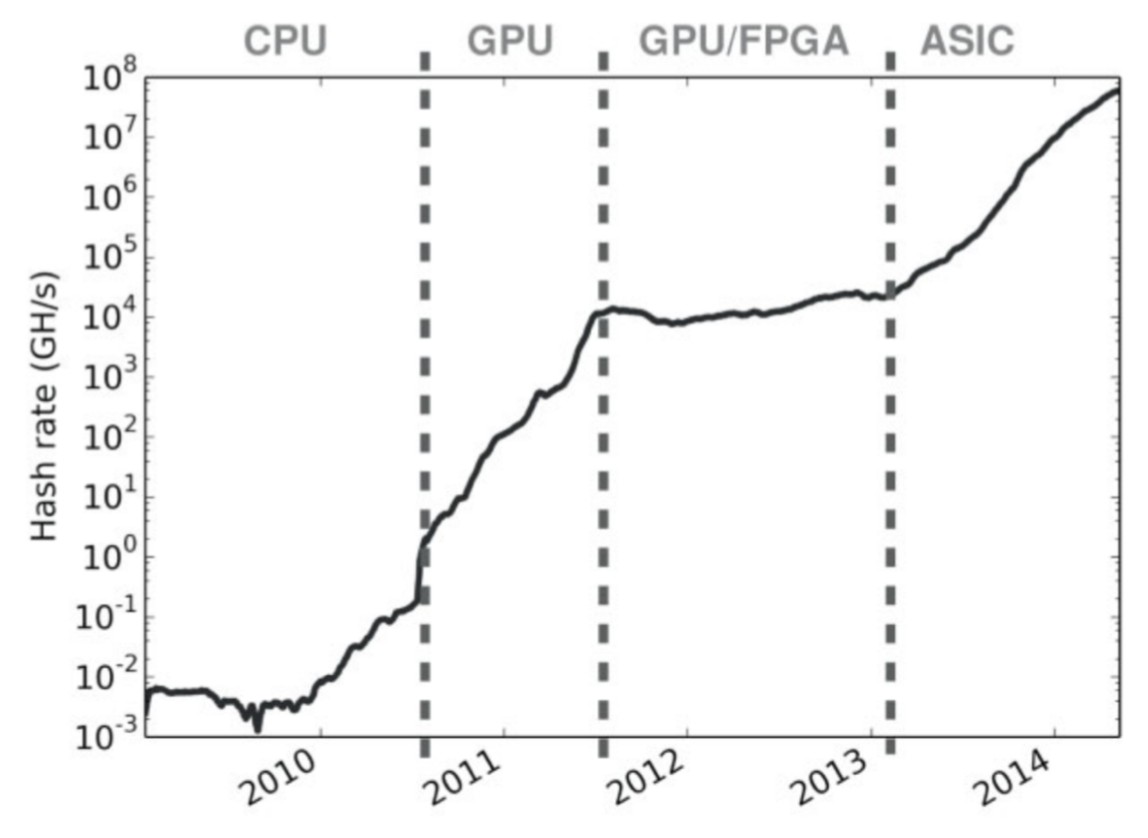
\includegraphics[width=8cm]{images/14.png}
    \caption{Mining technology comparison}
\end{figure}

\noindent There has been some controversy regarding the environmental impact of Bitcoin mining due to the total electricity consumption of the network. As mining technology catches up with state-of-the-art process technology, mining cost will be driven primarily by electricity costs and mining power will then probably shift to locations where electricity is cheaper. The environmental impact of electricity in places with low electricity costs might be smaller, as these are usually places with large natural sources of energy. Besides, the energy consumed by Bitcoin mining is arguably not wasted: it is employed in securing the blockchain.\newline
In the following sections, the environmental impact topic will be exhaustively analyzed also providing interesting comparisons with other payment methods.

\subsection*{Pooled Mining}
Individual miners are subject to a high degree of uncertainty as to when they will mine a new block. To help miners manage this risk, mining pools started to appear at the end of 2010. A mining pool is an aggregation of miners, who contribute their hash power to the pool and share the mining rewards. By forming a pool, miners can have a much more predictable income stream to share among them. Revenue sharing in a mining pool is proportional to the hash rate contributed by each miner, minus a small fee charged by the pool operator, which is usually run for profit. An additional advantage is that miners participating in a pool do not have to keep a copy of the full blockchain or process all incoming transactions: it is enough for the pool operator to feed miners a copy of the block header.\newline
Concentration of mining in a few pools is generally viewed as problematic by the Bitcoin community. The problem is that concentration makes it easier, and more profitable, to attempt attacks against other miners. Another potential problem stemming from mining concentration is that, as miners choose which transactions to include in a block, pools have the power to censor particular transactions, for instance the transactions using funds from certain addresses, which would break the fungibility of Bitcoins.

\subsection*{Transaction Fees}
As we presented in the previous sections, the blockchain blocks have a limitation of roughly 1MB total size. The size of a transaction depends on the number of addresses that the transaction draws funds from and on the number of addresses that the funds are sent to.\newline
Miners have to choose which transactions to include in the block they are mining from their unconfirmed transactions’ memory pool. This is an optimization problem over the block size. Miners generally use a greedy algorithm to solve this problem. Candidate transactions are ordered by their fee-per-kilobyte ratio in descending order and chosen from this list. There might be scenarios under which miners would refuse to include transactions in the blocks that they are mining because of the “bigger blocks take longer to broadcast” problem: including more transactions in a block makes the block bigger, which takes the block longer to broadcast through the network, increasing the risk that another miner might simultaneously find and broadcast a competing block.\par\noindent
There is a minimum transaction fee in the protocol. The goal of this fee is to prevent denial-of-service attacks that could flood the network with transactions that pay no fee. The minimum transaction fee is currently set to 1000 Satoshis or 0.00001 Bitcoins.

\subsection*{Selfish Mining}
An attack called ‘selfish mining’ is when a miner works on a private branch, without disclosing it to the public network. As long as its private branch is longer that the public branch, he/she keeps mining on this branch. Eventually when the public branch is about to catch up, he/she makes its private branch public. This renders the actual public branch invalid, because all miners that follow the protocol will discard the public branch and will switch to the newly released private branch. The result is that all the work employed by miners working in the public branch is wasted. This yields an advantage to the selfish miner, because its effort on the private branch is not wasted. The selfish miner that follows this strategy is able to collect bigger rewards than those proportional to its share of the network hash rate. The strategy gives an advantage to the selfish miner by fooling the rest of the miners and making them waste their time. A negative consequence of the growth of a selfish mining pool is that it concentrates the control of mining. A group controlling the network can censor transactions, or factor out transactions already included in the blockchain. This is counter to the philosophy of openness and non-censorship that underpins Bitcoin. Another negative consequence of selfish mining is an increase in the uncertainty of confirmed transactions, which could lead to much longer confirmation times.

\clearpage

\section*{Environmental Impact}
As we spoilered earlier the machines performing the “work” (block mining) are consuming huge amounts of energy while doing so. The Bitcoin Energy Consumption Index was created to provide insight into this amount, and raise awareness on the unsustainability of the proof-of-work algorithm.\newline
The continuous block mining cycle incentivizes people all over the world to mine Bitcoin. As mining can provide a solid stream of revenue, people are very willing to run power-hungry machines to get a piece of it. Over the years this has caused the total energy consumption of the Bitcoin network to grow to epic proportions, as the price of the currency reached new highs. The entire Bitcoin network now consumes more energy than a number of countries, based on a report published by the International Energy Agency. If Bitcoin was a country, it would rank as shown below.

\begin{figure}[H]
    \centering
    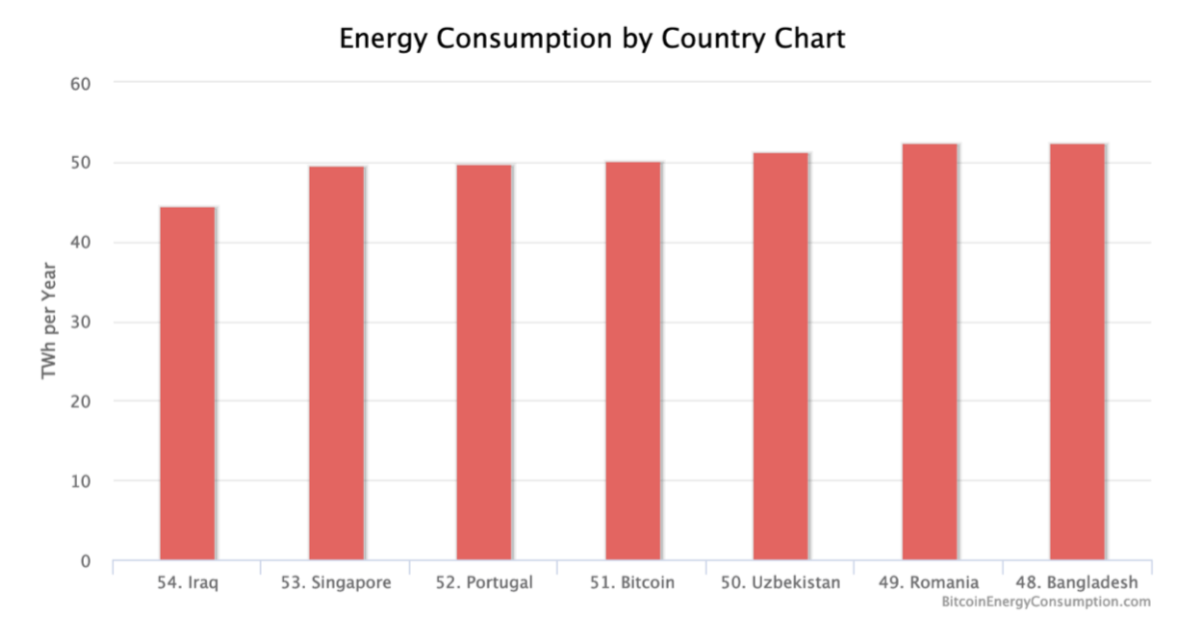
\includegraphics[width=12cm]{images/15.png}
    \caption{Bitcoin vs. coutries consumption}
\end{figure}

\noindent Bitcoin’s biggest problem is not even its massive energy consumption, but that the network is mostly fueled by coal-fired power plants in China. Even with a conservative emission factor, this results in an extreme carbon footprint for each unique Bitcoin transaction.\newline
To put the energy consumed by the Bitcoin network into perspective we can compare it to another payment system like VISA, that according to the company, all of its system consumed a total amount of 674,922 Gigajoules of energy (roughly equivalent to 17000 U.S. households) globally for all its operations. Since we also know that VISA processed 111.2 billion transactions in 2017 we can construct the direct comparison with the Bitcoin.

\begin{figure}[H]
    \centering
    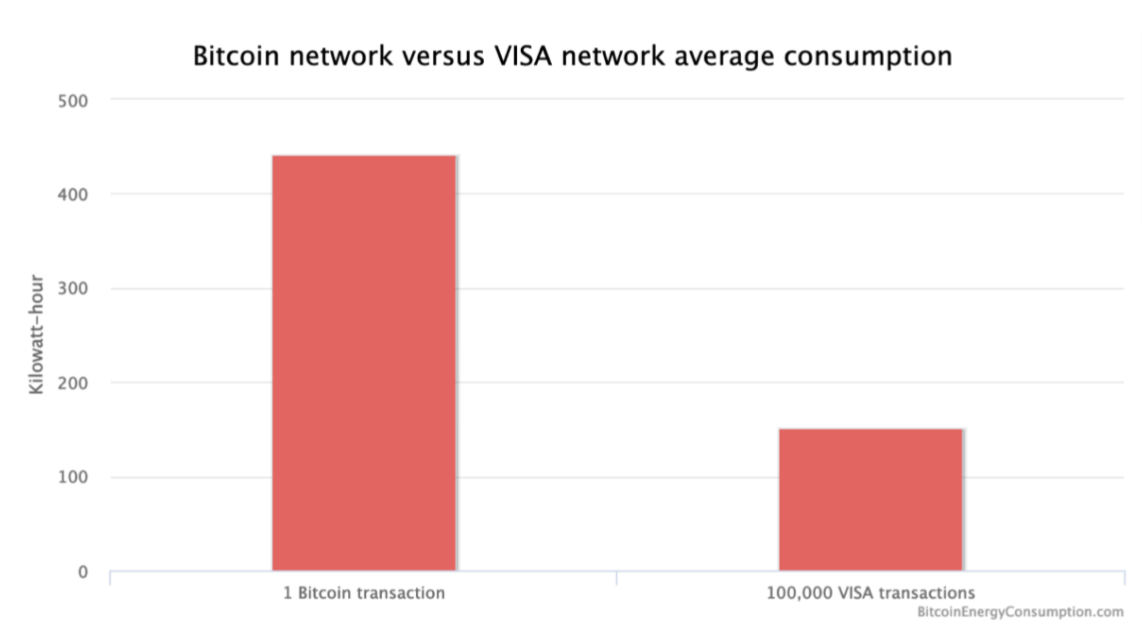
\includegraphics[width=10cm]{images/16.png}
    \caption{Bitcoin vs. VISA network consumption}
\end{figure}
\clearpage

\section*{Cracking Bitcoin Wallets}
Due to the increase of the Bitcoin value, more consumers are eagerly investing into its infrastructure. Consequently, there is also a corresponding increase in potential security threats and malicious actors. Due to the way Bitcoin and blockchain handle ownership, a user needs to have a Bitcoin address and Bitcoin wallet to prove title over the currency.\newline
The Bitcoin wallet is a single point of failure or attack vector for a malicious actor to gain control over an individual’s Bitcoins. There have been several high profile incidents where Bitcoin wallets were breached, resulting in losses amounting to millions of dollars. The only form of security in the Bitcoin wallet is a secret key that is given to every Bitcoin wallet. The downside to this implementation comes from the private key being stored in the Bitcoin wallet. If a malicious actor gains access to that Bitcoin wallet, then they can use that private key to gain control of that user’s Bitcoins. As we already said, the Bitcoin infrastructure uses the private key as the means of authenticating ownership of any Bitcoins owned by the associated Bitcoin address. If the private key is lost, so is all ownership.\par\noindent
In the recent years there has been a lot of studies on Bitcoin wallet security. One of the most relevant was an improved weighted threshold Elliptic Curve Digital Signature Algorithm (ECDSA) to secure Bitcoin wallets. The proposed algorithm distributes a part of the private key over a group of individuals. This provides additional security as no one individual has complete access. In the proposed approach, individuals are also separated into groups of differing weights, and each group has the same weight and a subset of players having more than or equal to a threshold value of that group can reconstruct the secret key.\newline
Another study demonstrated how introducing two-factor authentication to a Bitcoin wallet increases the security of it. However, the approach does not focus on protecting the password or data contained in the Bitcoin wallet itself from dedicated attacks.

\subsection*{Possible Attacks}
In the ``Cracking Bitcoin Wallets" [2] paper some researchers analyzed an attack performed against a wallet desktop application hosted on the user’s personal computer, with a 12-seed passphrase suggested by the wallet at the time of creation. The user may access the funds using either the password generated or the 12-seed passphrase (a combination of 12/24 words from a cluster of 2100 dictionary words encrypted in the wallet application).\par\noindent
The first step to archive the attack was to setup and create the software package for cracking the wallet words. The available option to crack through a wallet was to identify the dictionary and try all possible combinations (brute forcing). The above identified solution involved the following steps:
\begin{itemize}
    \item Extract the dictionary;
    \item Create the combinations for a dictionary file;
    \item Check for the correct passphrase.
\end{itemize}
The process opted to crack the passphrase was an offline brute force attack, which is a trial-and-error model and time consuming. It involves the trying of all possible combinations of characters in a sequence to crack an encrypted gateway. The implementation of the offline brute force attack used the extracted set of 2100 words (‘dataset’) from the wallet application.\par
\noindent Brute-forcing a 12 characters string means that for the each character there are 26 possibilities, since there are 26 letters in the English alphabet, and all of this results in \(26^{12} = 9.54 \cdot 10^{16}\) combinations. Now imagine when there are 2048 words that can potentially be used in a 12-word seed, then this would result to \(2052^{12} = 5.44 \cdot 10^{39}\) combinations. Now if 10 billion passwords are checked per second, it would take more than \(1.7 \cdot 10^{22}\) years to try all possibilities.\par\noindent
The attack described was able to identify more than one combination of a given 12 words (Seed) successfully using a normal desktop computer (limited computational power). The percentage of the identified valid combinations gradually decreases as the number of combinations fed to the application increases (the number of combinations valid for the dictionary feed given is between 1.01\% and 10\% for a given 12-word seed). Therefore, we can state the comfort levels of an attacker to exploit this vulnerability with a reasonable computational power (e.g. multiple servers or virtual machines) to acquire unauthorized access to the wallets.
\clearpage

\shipout\null

\section*{References}
\begin{enumerate}
    \item Antonino Salibra. \textit{Slides of the ``Cryptography Foundation" Ca' Foscari University master's degree course in ``Software Dependability and Cyber Security"} - 2019.
    \item Pedro Franco (Wiley). \textit{``Understanding Bitcoin, Cryptography, Engineering and Economics"} - 2015.
    \item Andreas M. Antonopoulos (O’Reilly). \textit{``Mastering Bitcoin - Programming the open blockchain"} - 2017.
    \item Tejaswi Volety, Shalabh Saini, Thomas McGhin, Charles Zhechao Liu, Kim-Kwang Raymond Choo. \textit{Elsevier, Future Generation Computer Systems - ``Cracking Bitcoin Wallets: I want what you have in the wallets"} - 2019.
    \item Eric Rykwalder (Coindesk). \textit{\href{https://www.coindesk.com/math-behind-bitcoin}{``The Math Behind Bitcoin"}} - 2014.
    \item Digiconomist. \textit{\href{https://digiconomist.net/bitcoin-energy-consumption}{``Bitcoin Energy Consumption Index"}}.
\end{enumerate}
\clearpage

\listoffigures

\end{document}